\documentclass[../main/main.tex]{subfiles}

\raggedbottom

\makeatletter
\renewcommand{\@chapapp}{Architecture de la mati\`ere -- chapitre}
\makeatother

\begin{document}
\setcounter{chapter}{1}

\chapter{Propri\'et\'es physico-chimiques macroscopiques}

À température ambiante, le dichlore est gazeux, le dibrome est liquide et le
diiode solide~: il y a donc des interactions qui expliquent la cohésion des
molécules entre elles malgré l'agitation thermique. Le but de ce chapitre est de
lister les forces intermoléculaires pour comprendre la cohésion de la matière.

\section{Interactions de \textsc{Van der Waals}}

Les interactions de \textsc{Van der Waals} regroupent trois types d'interactions
électrostatiques \textbf{attractives et additives} entre les molécules. Toutes
ces forces sont donc attractives, et diminiuent très rapidement avec la distance
entre les molécules. L'énergie potentielle d'interaction entre deux molécules
séparées d'une distance $d$ est de la forme
\[\boxed{\Ec_{p,VdW} = -\frac{\cte}{d^6}}\]

\subsection{Interaction dipôle/charge}

Physiquement, un moment dipolaire traduit une dissymétrie de charges entre deux
«~extrémités~» d'une molécule. Cette dissymétrie rend la molécule capable
d'interagir avec d'autres charges, voir figure~\ref{fig:dipq}~: très
schématiquement, une charge positive placée à proximité de la molécule est
globalement attirée par l'extrémité chargée $\de-$ et globalement repoussée par
l'extrémité chargée $\de+$. C'est bien sûr le contraire pour une charge
négative.

\begin{figure}[H]
    \centering
    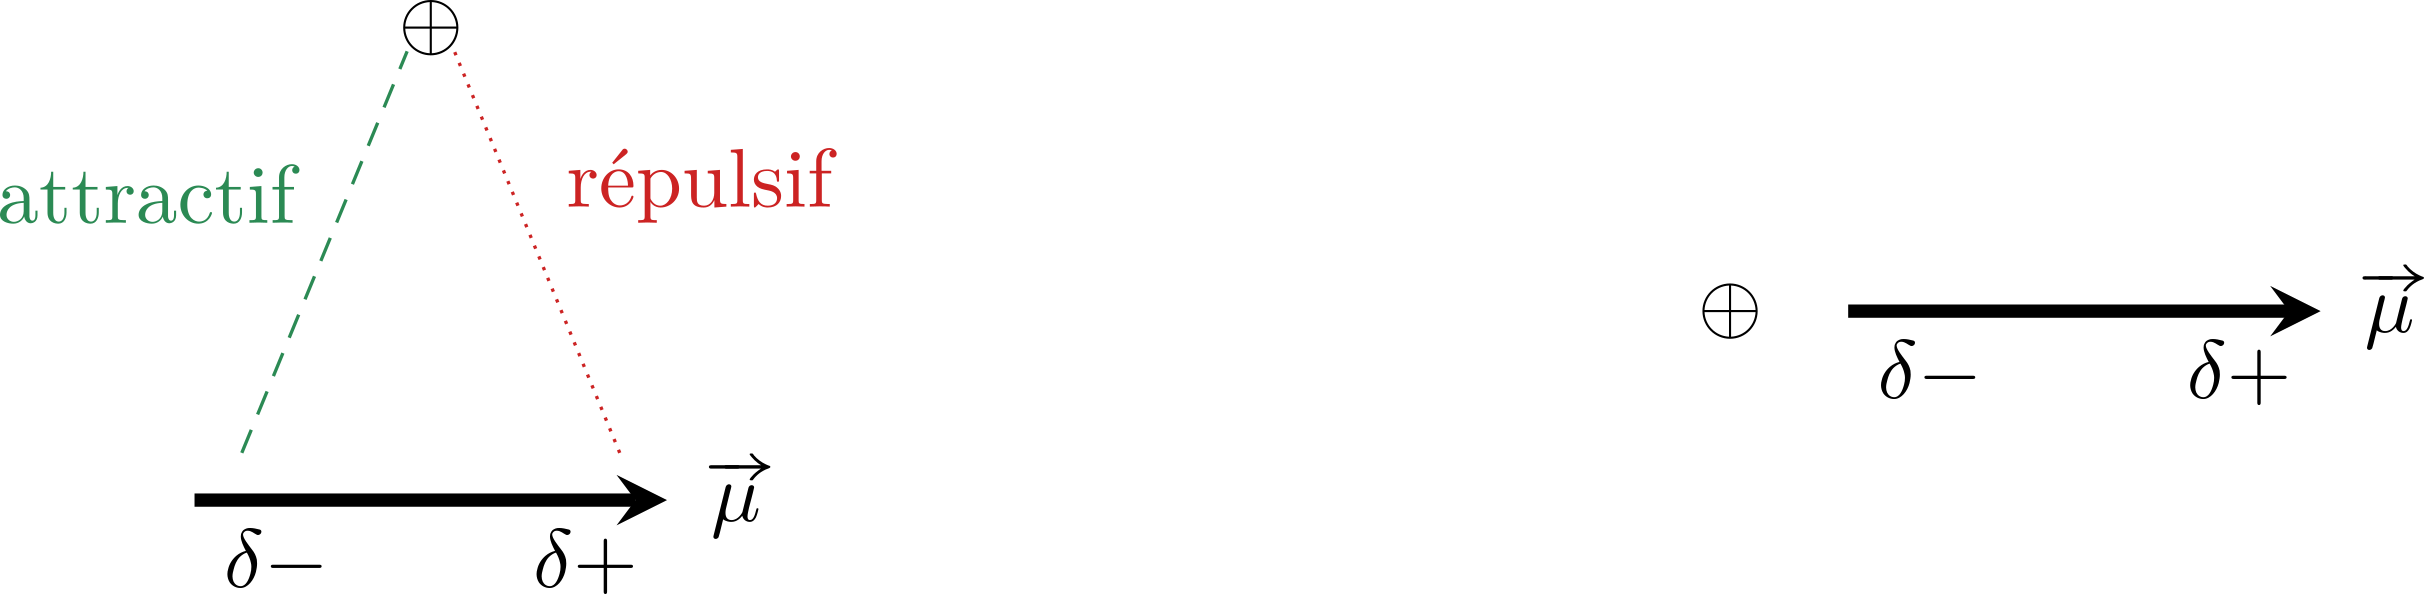
\includegraphics[scale=1]{dipq}
    \caption{Interaction électrostatique entre un dipôle et une charge.}
    \label{fig:dipq}
\end{figure}

\subsection{Interaction de \textsc{Keesom}~: permanent/permanent}

Le mécanisme discuté précédemment se généralise aux cas d'une interaction entre
deux dipôles, voir figure~\ref{fig:keesom}~: la charge $\de-$ du dipôle 2 tend à se
placer derrière la charge $\de+$ du dipôle 1, et réciproquement. On peut alors
montrer que la position d'équilibre du dipôle 2 est celle où il est aligné avec
le dipôle 1.

\begin{figure}[H]
    \centering
    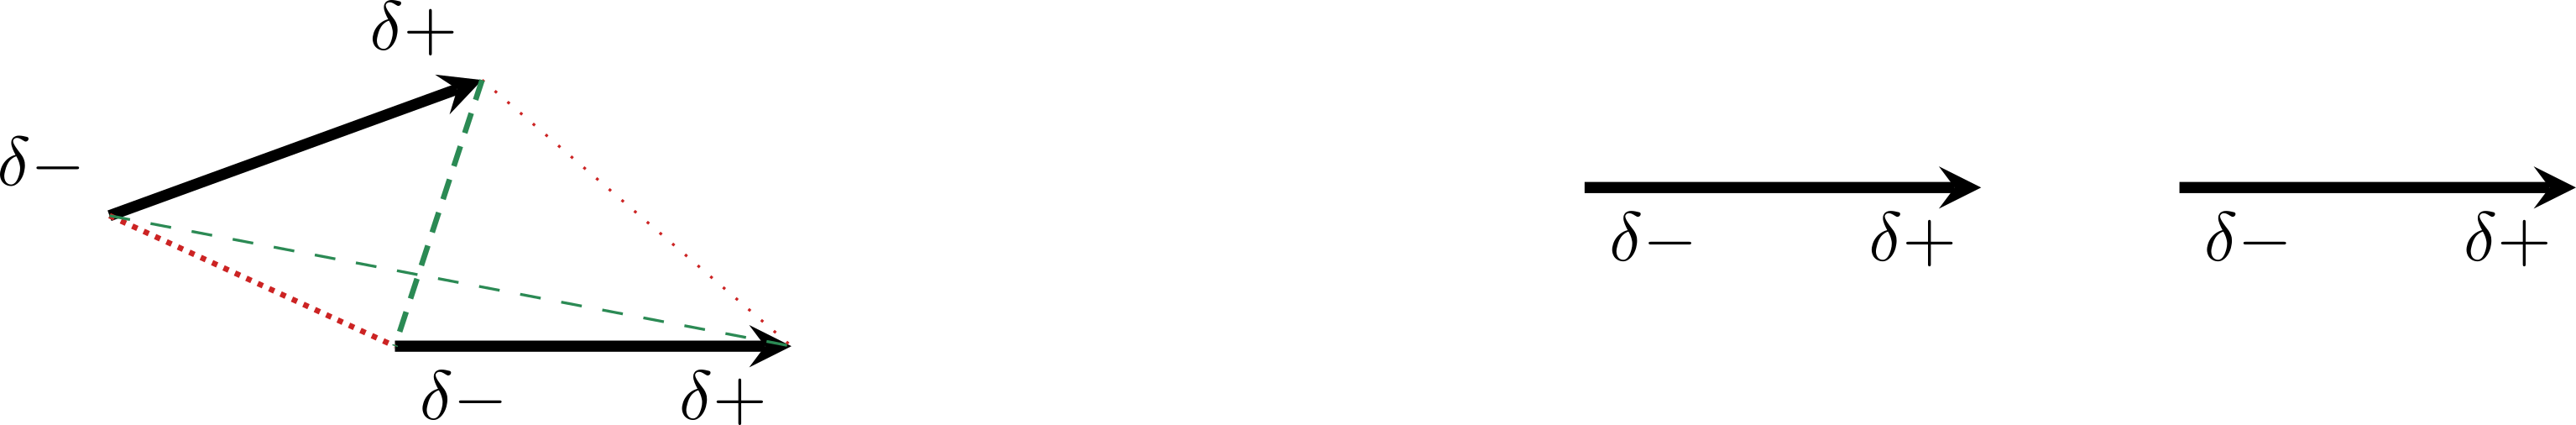
\includegraphics[scale=1]{keesom}
    \caption{Interaction de \textsc{Keesom} entre deux dipôles permanents}
    \label{fig:keesom}
\end{figure}

Ce mécanisme d'interaction entre deux dipôles permanents définit l'interaction
de \textsc{Keesom,} qui fait partie des interactions de \textsc{Van der Waals}. On peut
résumer ses propriétés~:
\begin{itemize}[label=$\diamond$]
    \litem{Nature}~: force entre 2 molécules polaires (dipôle permanent/dipôle
        permanent).
    \litem{Énergie potentielle}~:
        \[\Ec_p = -k \frac{\mu_{\ce{A}}{}^2\mu_{\ce{B}}{}^2}{d^6}\]
        avec $\mu_{\ce{A}}$ et $\mu_{\ce{B}}$ les moments dipolaires de A et B, $k$
        une constante physique (dépendant de $T$).
    \litem{Énergie de liaison}~: \SIrange{0.5}{3}{kJ.mol^{-1}}.
\end{itemize}

L'énergie d'une liaison de correspond à l'énergie nécessaire pour pour casser
\SI{1}{mol} de liaisons.

\subsection{Interaction de \textsc{Debye}~: permanent/induit}

Comme introduit dans le chapitre précédent, les molécules ne sont pas des
solides mais peuvent se déformer, en particulier sous l'effet des forces de
Coulomb subies par les noyaux et les électrons. Cette capacité est traduite par
la \textbf{polarisabilité}, dont on rappelle les caractéristiques ici~:
\begin{timpo}{Rappel~: polarisabilité}
    La capacité qu'a le nuage électronique d'une molécule de se déformer est
    quantifiée par sa polarisabilité, nombre sans dimension souvent noté $\a$.
    En général, une molécule est d'autant plus polarisable qu'elle est
    «~volumineuse~», ce qui est souvent équivalent à dire que sa masse
    molaire/son numéro atomique est élevé(e).
\end{timpo}

Ainsi, lorsqu'une molécule polaire se trouve à proximité d'une molécule
apolaire, le nuage électronique de la molécule apolaire se déforme. La figure 3
représente très schématiquement un exemple d'une telle situation~: un excès de
charge négative $\de'-$ se forme au voisinage de la charge partielle $\de+$ de
la molécule polaire. Finalement, la molécule initialement apolaire acquiert à
son tour un moment dipolaire $\pf_{\rm ind}$~: on parle de moment dipolaire
\textbf{induit}, ou dipôle induit. Ce dipôle induit interagit alors avec le
dipôle permanent de l'autre molécule comme pour l'interaction de
\textsc{Keesom}~: cette interaction particulière est celle dite de
\textsc{Debye}.

\begin{figure}[H]
    \centering
    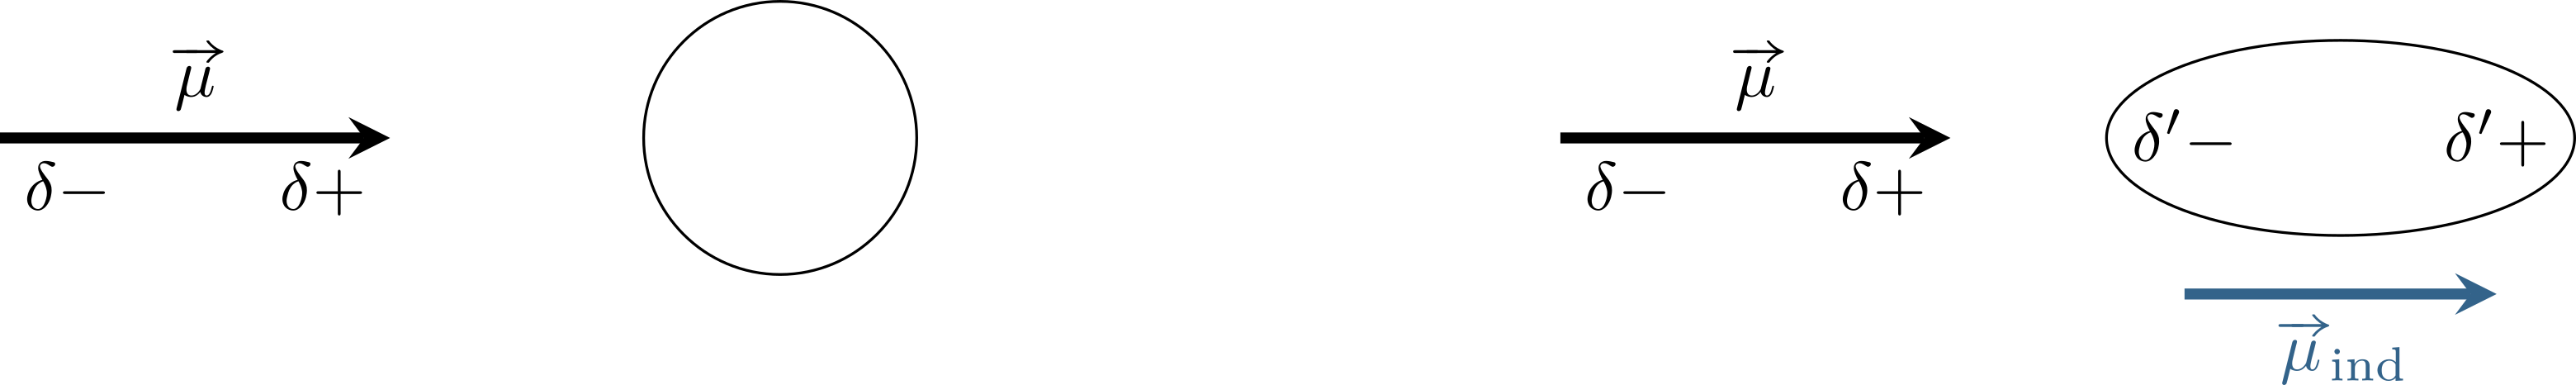
\includegraphics[scale=1]{debye}
    \caption{Interaction de \textsc{Debye} entre un dipôle permanent et un
    dipôle induit.}
    \label{fig:debye}
\end{figure}

Ainsi, pour l'interaction de \textsc{Debye}~:
\begin{itemize}[label=$\diamond$]
    \litem{Nature}~: force entre 1 molécule polaire et 1 apolaire (dipôle
        permanent/dipôle induit).
    \litem{Énergie potentielle}~:
        \[\Ec_p = -k' \frac{\mu_{\ce{A}}{}^2\a_{\ce{B}}}{d^6}\]
        avec $\mu_{\ce{A}}$ le moment dipolaire de A et $\a_{\ce{B}}$ la
        polarisabilité de B, $k'$ constante (dépend de $T$).
    \litem{Énergie de liaison}~: \SIrange{0.02}{0.5}{kJ.mol^{-1}}.
\end{itemize}
L'effet est donc en général plus faible que celui des interactions de Keesom.

\subsection{Interaction de \textsc{London}~: induit/induit}

Enfin, même si elle est globalement apolaire, le mouvement incessant des
électrons fait qu'une molécule possède toujours un moment dipolaire instantané
(c'est une image~: le moment dipolaire instantané est d'origine quantique).
Comme attendu, ce moment dipolaire instantané est d'autant plus grand que la
molécule est polarisable. Ces moments dipolaires peuvent ensuite interagir entre
eux, ce qui se traduit globalement par une interaction attractive entre les
molécules, appelée interaction de \textbf{London}, qui fait partie des
interactions de \textsc{Van der Waals}.

\begin{itemize}[label=$\diamond$]
    \litem{Nature}~: force entre 2 molécules apolaires (dipôle induit/dipôle
        induit).
    \litem{Énergie potentielle}~:
        \[\Ec_p = -k'' \frac{\a_{\ce{A}}\a_{\ce{B}}}{d^6}\]
        avec $\a_{\ce{A}}$ et $\a_{\ce{B}}$ la polarisabilité de A et B, $k''$
        une constante physique (dépendant de $T$).
    \litem{Énergie de liaison}~: \SIrange{0.5}{30}{kJ.mol^{-1}}.
\end{itemize}

Les interactions de London sont donc en général largement dominantes sur les
deux autres, contrairement à ce que l'on pourrait croire à première vue.

\subsection{Bilan et comparaison}

\begin{table}[h!]
    \centering
    \caption{Comparaison des propriétés des interactions de \textsc{Van der
    Waals}.}
    \label{tab:vdwcomp}
    \begin{tabular}{ccccc}
        \toprule
        Nom & Type d'interaction & Condition d'existence & Nature & Énergie de
        liaison
        \\\midrule
        \textsc{Keesom} & permanent-permanent & molécules polaires & attractive
                        & \SI{1}{kJ.mol^{-1}}
        \\
        \textsc{Debye} & permanent-induit & une polaire, une polarisable & attractive
                        & \SI{0.1}{kJ.mol^{-1}}
        \\
        \textsc{London} & induit-induit & molécules polarisables & attractive
                        & \SI{10}{kJ.mol^{-1}}
        \\\bottomrule
    \end{tabular}
\end{table}

\begin{itemize}[label=$\diamond$]
    \item Les interactions de \textsc{Van der Waals} sont toujours attractives.
    \item L'énergie d'une liaison de \textsc{Van der Waals} est de l'ordre de
        quelques kilojoule par mole, soit cent fois moins qu'une liaison
        covlante~: on les qualifie de liaisons faibles.
    \item Plus une liaison est faible, plus la longueur de liaison est grande~:
        deux molécules «~liées~» entre elles par une liaison de \textsc{Van der
        Waals} sont malgré tout relativement éloignées l'une de l'autre.
    \item Comme toutes les molécules sont polarisables, toutes sont sujettes aux
        interactions de \textsc{Van der Waals}. Plus la masse molaire d'une
        molécule est élevée, plus sa polarisabilité $\a$ augmente.
\end{itemize}

\begin{table}[h!]
    \centering
    \caption{Contributions relatives des trois interactions de \textsc{VdW} à
    l'énergie totale.}
    \label{tab:vdwcont}
    \begin{tabular}{cccccc}
        \toprule
        \multirow{2}{*}[-3pt]{Espèce} &
        \multirow{2}{*}[-3pt]{Moment dipolaire (\si{D})} &
        \multirow{2}{*}[-3pt]{Polarisabilité} &
        \multicolumn{3}{c}{Contributions relatives (\%)}
        \\\cmidrule{4-6}
        & & &
        \textsc{Keesom} & \textsc{Debye} & \textsc{London}
        \\\midrule
        \ce{He} & 0 & \num{0.2} & 0 & 0 & 100
        \\
        \ce{H2} & 0 & \num{0.79} & 0 & 0 & 100
        \\
        \ce{H2O} & \num{1.85} & \num{1.48} & 69 & 7 & 24
        \\
        \ce{NH3} & \num{1.47} & \num{2.22} & 34 & 9 & 57
        \\
        \ce{HCl} & \num{1.08} & \num{2.63} & 9 & 5 & 86
        \\
        \ce{HBr} & \num{0.79} & \num{3.61} & 2 & 2 & 96
        \\
        \bottomrule
    \end{tabular}
\end{table}

\subsection{Forces répulsives}
En ne considérant que les interactions de \textsc{Van der Waals}, les molécules
devraient donc s'attirer jusqu'à $d=0$, ce qui n'est pas le cas~: la matière ne
s'effondre pas. En réalité, \textbf{il existe des forces répulsives} et qui
compensent les forces de \textbf{VdW} à très courte distance. Elles sont dues au
fait que les nuages électroniques ne peuvent s'interpénétrer. Elles sont
associées à une énergie potentielle de répulsion~:
\[\Ec_p = + \frac{B}{d^{12}}\]
d'où l'énergie potentielle totale, tracée figure~\ref{fig:eprep}~:
\[
    \Ec_p =
        \underbracket[1pt]{-\frac{A}{d^6}}_{\text{attraction}}
        \underbracket[1pt]{+\frac{B}{D^{12}}}_{\text{répulsion}}
\]

\begin{figure}[h!]
    \centering
    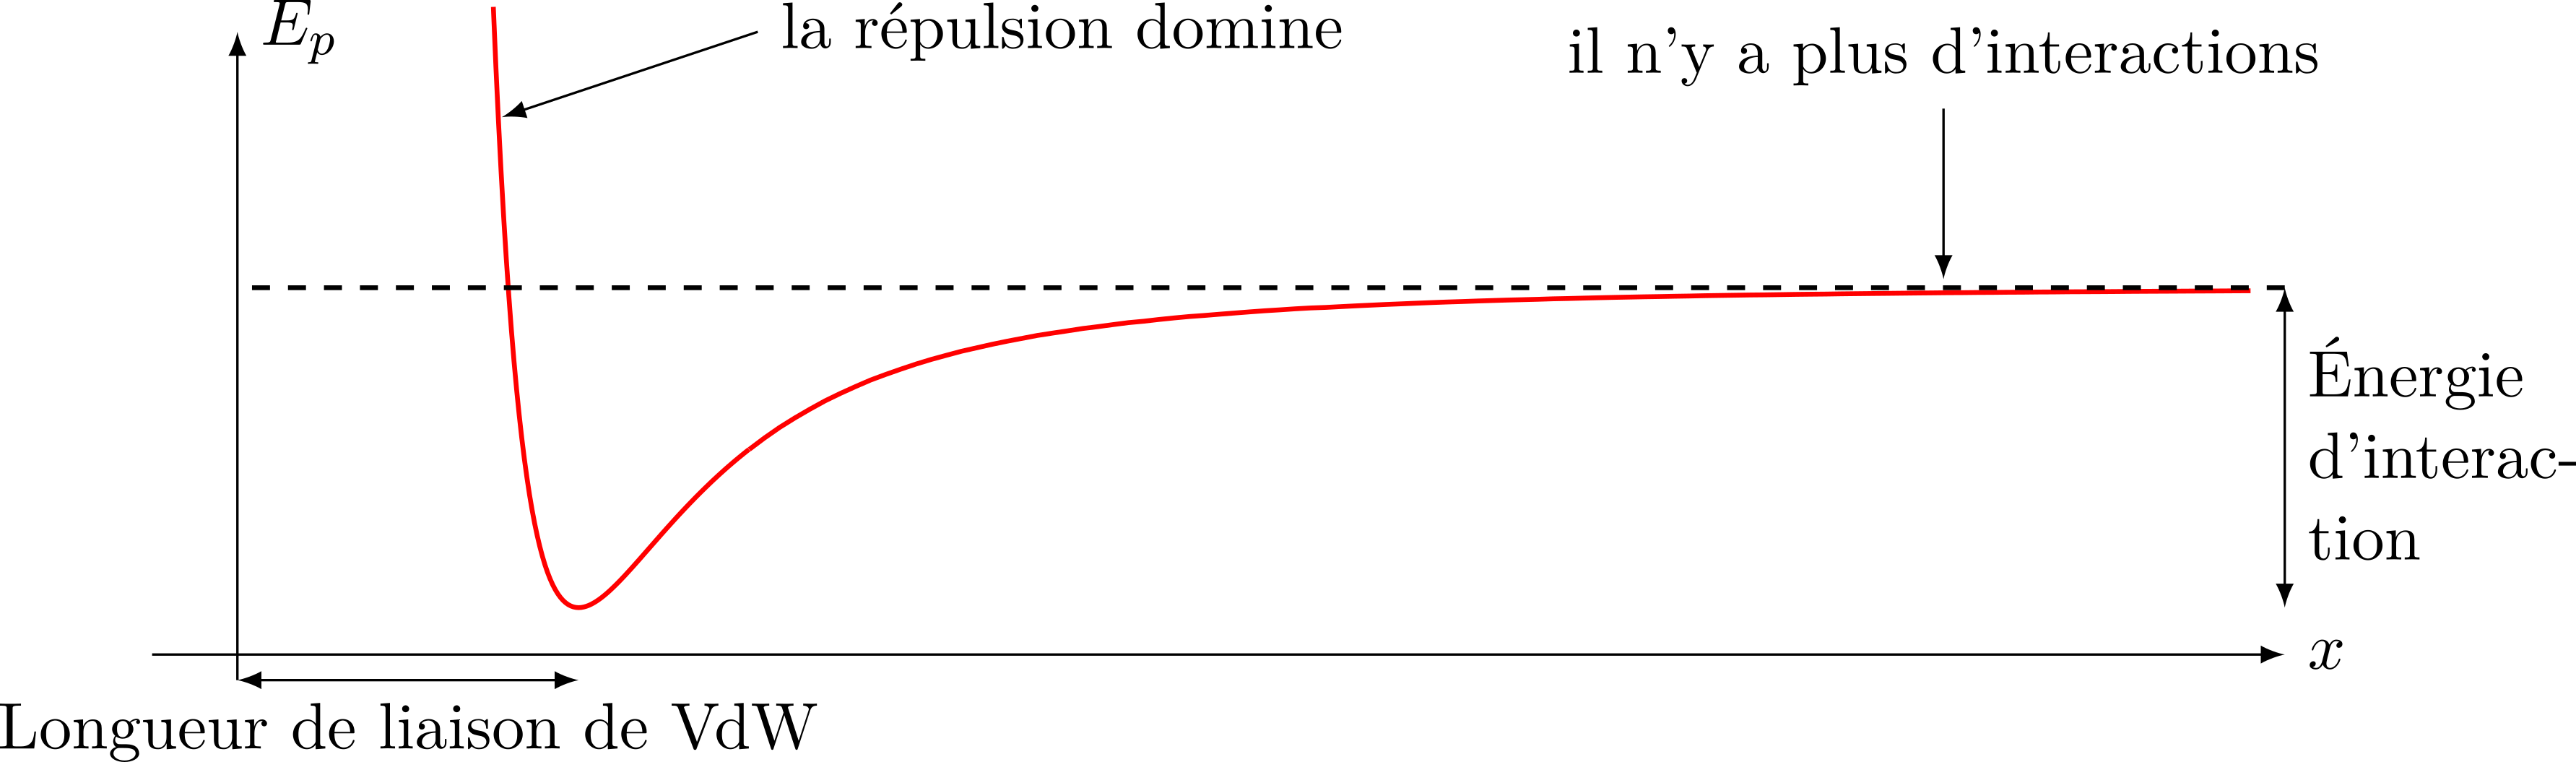
\includegraphics[scale=1]{eprep}
    \caption{Forme de l'énergie potentielle totale d'interaction entre deux
    molécules. La première est supposée fixée en $x=0$, et la seconde se situe à
une distance $x$ d'elle. Le puits de potentiel montre la position d'équilibre
stable, quand la dérivée de l'énergie potentielle est nulle~: à cette position,
la distance intermoléculaire et fixe, c'est la longueur de liaison. L'énergie de
liaison correspond à l'énergie à fournir à la molécule au fond du puits pour
l'amener à un état de diffusion, au-dessus de la ligne en pointillés.}
    \label{fig:eprep}
\end{figure}
L'énergie totale est attractive à longue distance, mais répulsive à très courte
distance. La distance d'équilibre est autour de \SIrange{300}{500}{pm}.

\section{Températures de changement d'état}
La température d'un changement d'état résulte de la compétition entre deux
énergies~:
\begin{itemize}
    \item D'une part l'énergie thermique, de l'ordre de $RT$ ($\approx
        \SI{2.5}{kJ.mol^{-1}}$ à $T_{\rm ambiant}$~;
    \item D'autre part l'énergie de cohésion liée aux interactions de
        \textsc{VdW} ($\approx \SI{1}{kJ.mol^{-1}}$).
\end{itemize}
Chauffer un composant revient à donner suffisamment d'énergie cinétique à un
atome ou molécule pour qu'elle quitte le puits de potentiel qui la relie à un
autre atome ou molécule (voir Figure~\ref{fig:eprep}). Ainsi,
\begin{tror}{Conclusion, heart}
    \begin{center}
        \bfseries
        Plus les interactions attractives sont fortes, plus les températures de
        changement d'état sont élevées.
    \end{center}
\end{tror}

\subsection{Influence de la polarité}
\subsubsection{Exemple 1~: \ce{CO} et \ce{NO}}
\vspace{-10pt}
\begin{table}[h!]
    \centering
    \caption{Caractéristiques de \ce{CO} et \ce{NO}.}
    \label{tab:cono}
    \begin{tabular}{ccc}
        \toprule
        Édifice & $\mu$ (\si{D}) & $\tt_{\rm eb}
        (\si{\degreeCelsius})$
        \\\midrule
        \ce{CO} & \num{0.112} & \num{-191.5}
        \\
        \ce{NO} & \num{0.153} & \num{-151.8}
        \\
        \bottomrule
    \end{tabular}
\end{table}
\vspace{-10pt}

\subsubsection{Exemple 2~: isomères du 1,2-chloroéthène}
\bigbreak
\begin{minipage}{0.49\linewidth}
    \begin{gather*}
        \cfig{
            @{Cg1}C
            (-[3]@{Clg1}Cl)
            (-[5]H)
            =_[@{mid1}0]@{Cd1}C
            (-[1]@{Cld1}Cl)
            (-[7]H)
        }
        \chemmove[red, -stealth]{
            \draw
            (mid1) --++
            (0,50pt)
            node [right] {$\muf$};
            \draw[transform canvas={xshift=4pt, yshift=4pt}, -stealth]
            (Cg1) --
            node [midway, above, sloped] {$\muf_{\ce{CCl}}$}
            (Clg1);
            \draw[transform canvas={xshift=-4pt, yshift=4pt}, -stealth]
            (Cd1) --
            node [midway, above, sloped] {$\muf_{\ce{CCl}}$}
            (Cld1);
        }
        \\
        \text{(Z)-1,2-dichloroéthène}
        \\
        \tt_{\rm eb} = \SI{60}{\degreeCelsius}
    \end{gather*}
\end{minipage}
\hfill
\begin{minipage}{0.49\linewidth}
    \begin{gather*}
        \cfig{
            @{Cg2}C
            (-[3]H)
            (-[5]@{Clg2}Cl)
            =_[@{mid2}0]@{Cd2}C
            (-[1]@{Cld2}Cl)
            (-[7]H)
        }
        \chemmove[red, -stealth]{
            \node[below] at (mid2) {$\muf = \of$};
            \draw[transform canvas={xshift=-4pt, yshift=2pt}, -stealth]
            (Cg2) --
            node [midway, above, sloped] {$\muf_{\ce{CCl}}$}
            (Clg2);
            \draw[transform canvas={xshift=-4pt, yshift=4pt}, -stealth]
            (Cd2) --
            node [midway, above, sloped] {$\muf_{\ce{CCl}}$}
            (Cld2);
        }
        \\
        \text{(E)-1,2-dichloroéthène}
        \\
        \tt_{\rm eb} = \SI{48}{\degreeCelsius}
    \end{gather*}
\end{minipage}
Ici aussi, l'interaction de \textsc{London} est du même ordre pour les deux
espèces (même taille $\Ra \approx$ même polarisabilité)~; par contre, les
interactions de \textsc{Keesom} et \textsc{Debye} ajoutent de la cohésion pour
la première espèce.

\subsubsection{Conclusion}
On observe ici~:
\begin{tror}{Observation, hand}
    Plus le \textbf{moment dipolaire est grand}, plus les espèces ont une forte
    cohésion, et donc plus la \textbf{température} de changement d'état est
    \textbf{élevée} (à polarisabilité proche).
\end{tror}

\subsection{Influence de la polarisabilité}
\subsubsection{Exemple 1~: composés hydrogénés de la 14\ieme\ colonne}
On observe l'évolution suivante pour les températures d'ébullition des composés
hydrogénés de la 14\ieme\ colonne~: \smallbreak
\begin{minipage}{0.50\linewidth}
    \begin{center}
        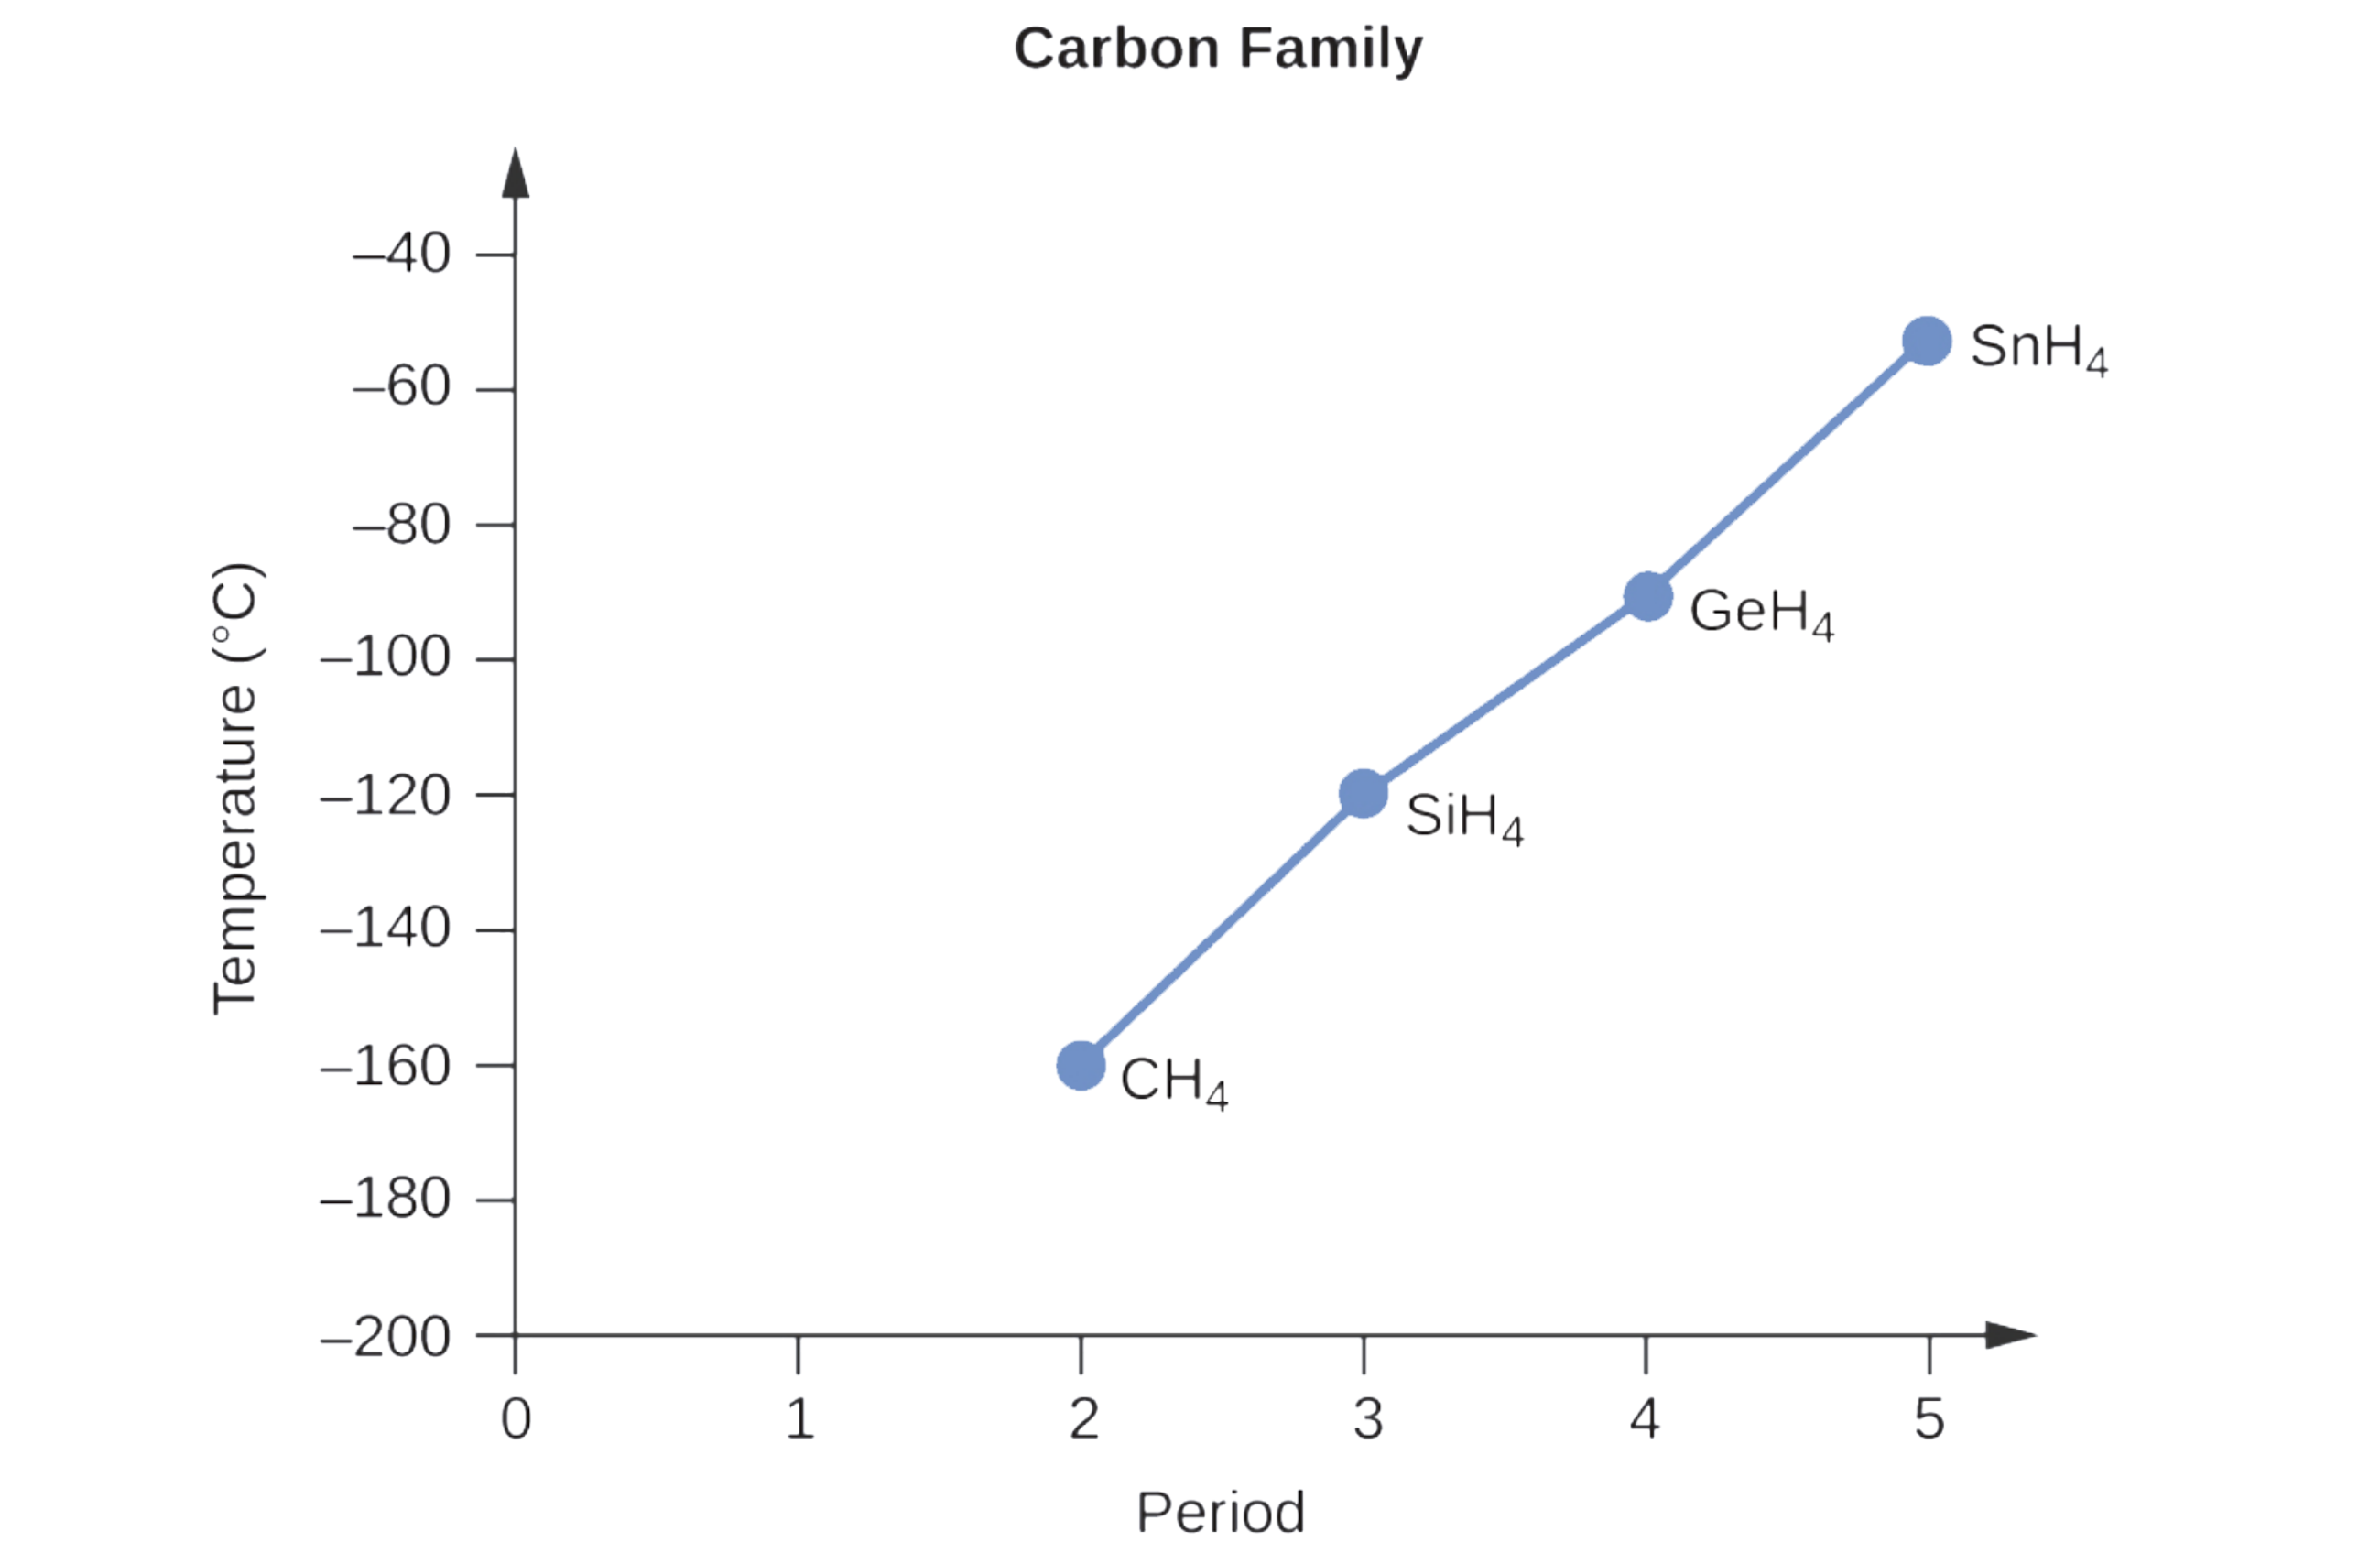
\includegraphics[width=\linewidth]{polarex}
    \end{center}
\end{minipage}
\hfill
\begin{minipage}{0.45\linewidth}
    Le nuage électronique devient plus gros lorsque l'on va vers le bas,
    l'interaction de \textsc{London} croît, la température d'ébullition croît (les
    molécules sont très peu polaires, les autres interactions sont
    quasi-inexistantes).
\end{minipage}

\subsubsection{Exemple 2~: dihalogènes}
\begin{table}[h!]
    \centering
    \caption{Températures de changement d'état pour des dihalogènes.}
    \label{tab:dihaltemp}
    \begin{tabular}{ccc}
        \toprule
        Édifice & $\tt_{\rm fus} (\si{\degreeCelsius})$ & $\tt_{\rm eb}
        (\si{\degreeCelsius})$
        \\\midrule
        \ce{Cl2} & \num{-102} & \num{-34}
        \\
        \ce{Br2} & \num{-7} & \num{59}
        \\
        \ce{I2} & \num{113} & \num{185}
        \\
        \bottomrule
    \end{tabular}
\end{table}
La molécule de diiode est plus polarisable que celle du dibrome, elle-même plus
polarisable que celle de dichlore. Les interactions de \textsc{London} est donc
plus importante, la cohésion plus élevée et la température de fusion ou
d'ébullition plus élevée.

\subsubsection{Conclusion}
\begin{tror}{Observation, hand}
    Plus une molécule est \textbf{polarisable}, c'est-à-dire grande en taille,
    plus les températures de changement d'état sont \textbf{élevées}.
\end{tror}

\section{Liaison hydrogène}
\subsection{Introduction}
La polarisabilité décroît notablement lorsque l'on remonte une colonne du
tableau périodique~; ainsi, en considérant les interactions de \textsc{Van der
Waals}, on s'attend à ce que~:
\begin{itemize}
    \item \ce{NH3} bouille à $\approx \SI{-130}{\degreeCelsius}$~;
    \item \ce{HF} bouille à $\approx \SI{-120}{\degreeCelsius}$.
    \item \ce{H2O} bouille à $\approx \SI{-80}{\degreeCelsius}$~;
\end{itemize}
Or, ça n'est évidemment pas le cas.

\begin{minipage}[t]{0.45\linewidth}
    \begin{center}
        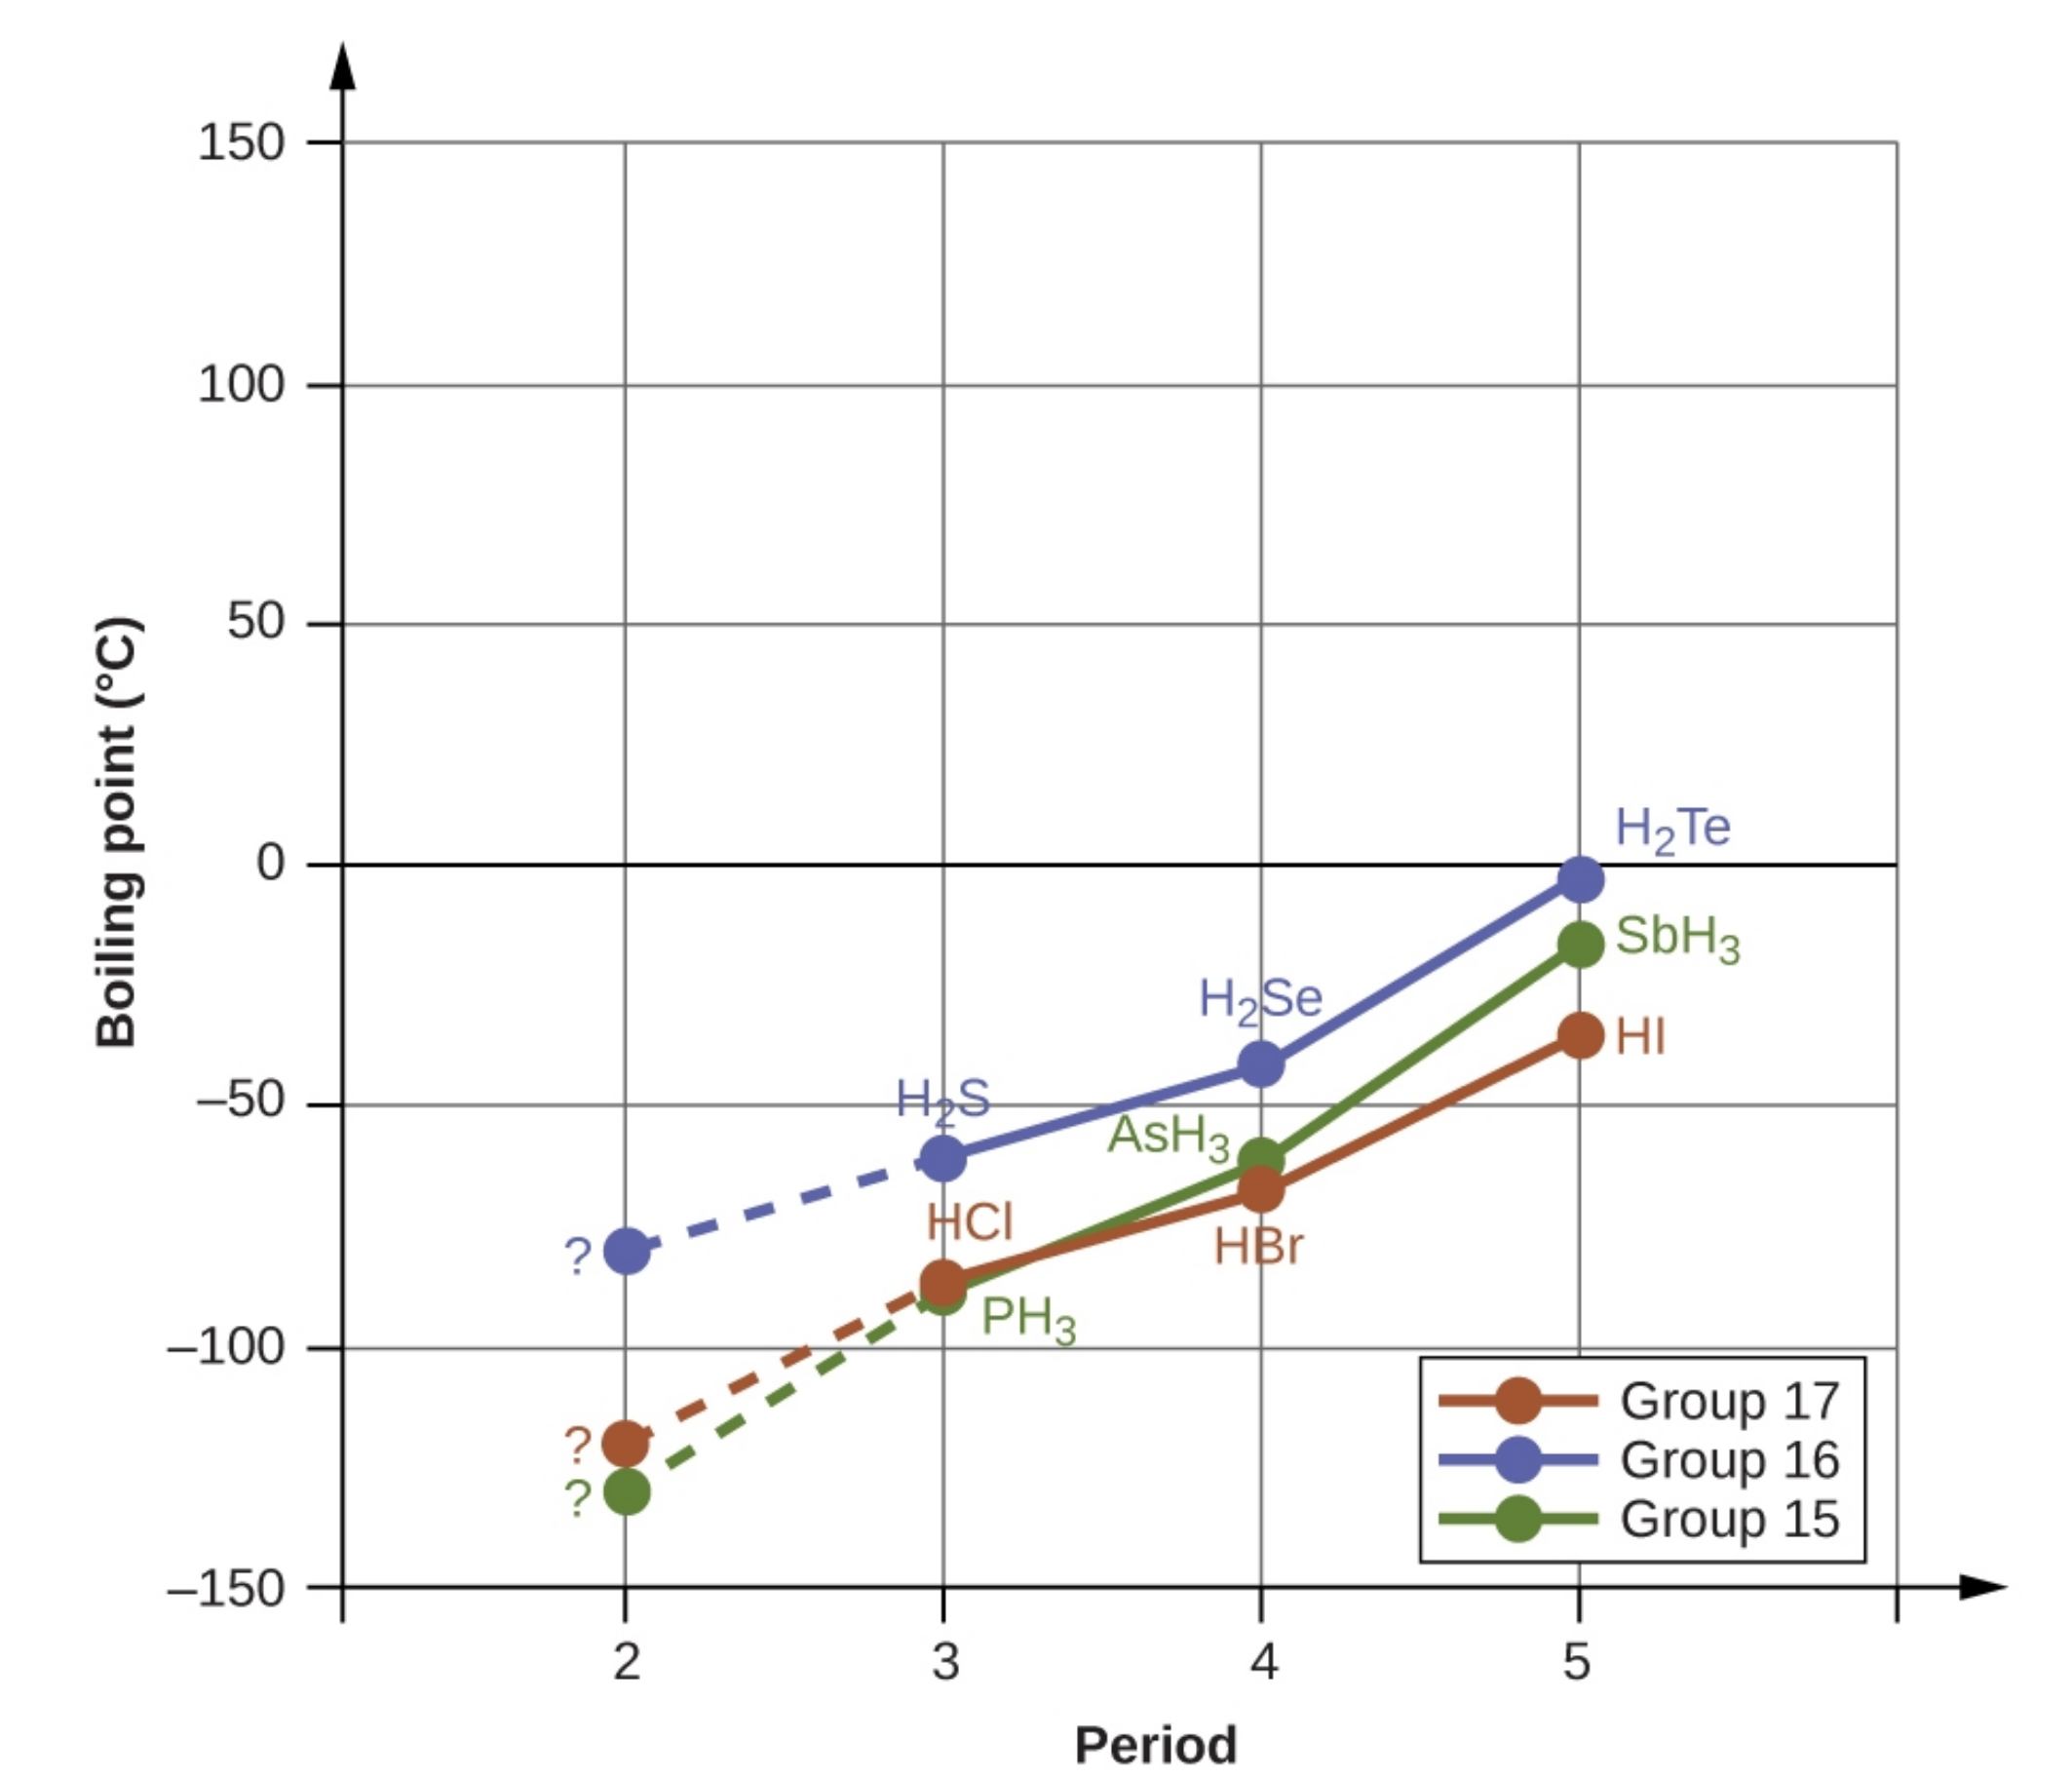
\includegraphics[width=\linewidth]{lhexp_a}
        \captionsetup{justification=centering}
        \captionof{figure}{Températures d'ébullition attendues.}
    \end{center}
\end{minipage}
\hfill
\begin{minipage}[t]{0.45\linewidth}
    \begin{center}
        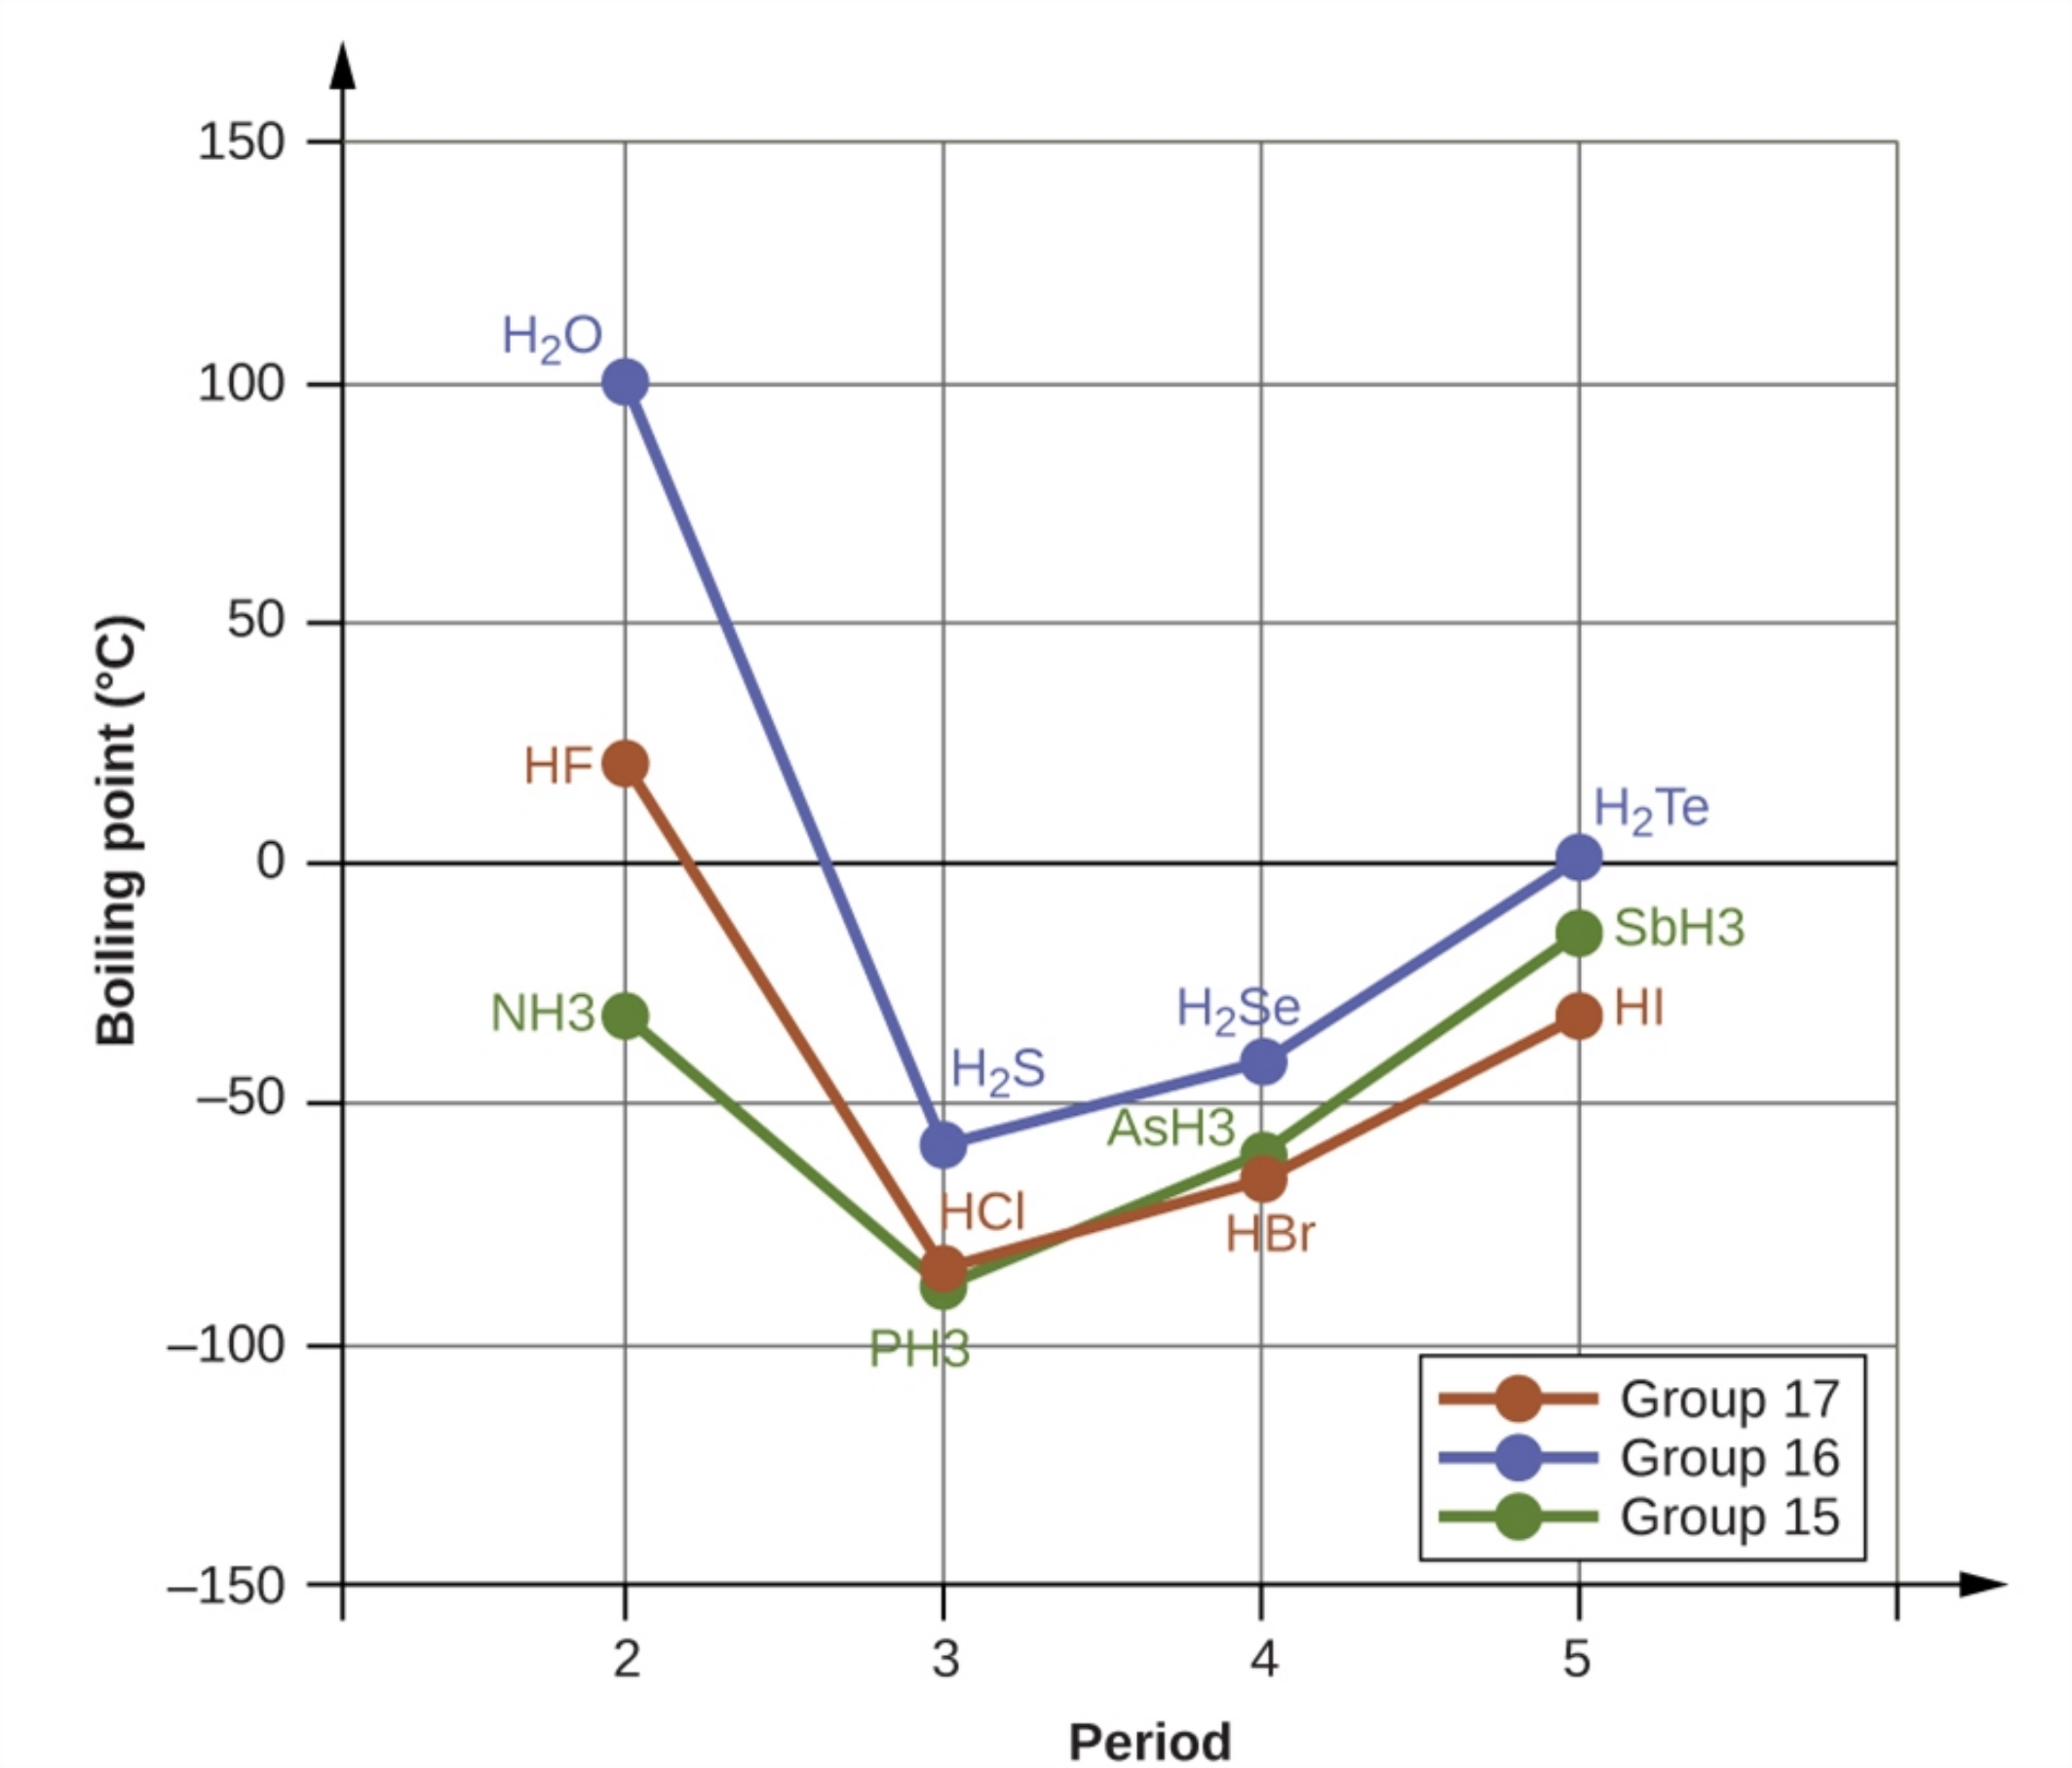
\includegraphics[width=\linewidth]{lhexp_b}
        \captionsetup{justification=centering}
        \captionof{figure}{Températures d'ébullition observées.}
    \end{center}
\end{minipage}

\medskip
La même chose se produit en comparant l'éthanol et le chloroéthane~:
\begin{table}[h!]
    \centering
    \caption{Comparaison des propriétés du chloroéthane et de l'éthanol.}
    \label{tab:chlocomp}
    \begin{tabular}{lccc}
        \toprule
        Nom & Représentation & $\mu$ (\si{D}) & $\tt_{\rm eb}
        (\si{\degreeCelsius})$
        \\\midrule
        Chloroéthane &
        \cfig{[,.5]
            C
            (-[2]\lewis{024,Cl})
            (-[4]H)
            (-[6]H)
            -C
            (-[0]H)
            (-[2]H)
            (-[6]H)
        } &
        \num{2.06} & \num{12}
        \\\midrule
        Éthanol &
        \cfig{[,.5]
            C
            (-[2]H)
            (-[4]H)
            (-[6]H)
            -C
            (-[2]H)
            (-[6]H)
            -\lewis{26,O}
            -H
        } &
        \num{1.71} & \num{60}
        \\\bottomrule
    \end{tabular}
\end{table}

On observe ici qu'en dépit d'une polarisabilité moindre et d'un moment dipolaire
plus faible, l'éthanol a une plus grande cohésion que le chloroéthane.

\subsection{Définition et exemples}
\begin{tdefi}{Définition~: liaison hydrogène, heart}
    Une \textbf{liaison hydrogène} s'établit en un atome d'hydrogène porté par
    un atome très électronégatif (\ce{N}, \ce{O} ou \ce{F}) et un autre atome
    \ce{B} également très électronégatif, porteur d'au moins un doublet
    non-liant et neutre. \bigbreak
    Autrement dit, la liaison hydrogène se fait entre un hydrogène dans une
    liaison ionisée et un doublet non-liant d'un atome électronégatif. Elle se
    représente par un trait pointillé.
    \begin{center}
        \cfig{
            \lewis{24,O}
            (-[6]H)
            (-[0]@{hg}H)
        }
        \hspace{1.5cm}
        \cfig{
            @{Oh}\lewis{24,O}
            (-[6]H)
            (-[0]H)
        }
        \chemmove[dashed, -]{
            \draw
            ([shift={(2pt,0)}]hg.east) --
            node [midway, above]
                {\scriptsize Liaison}
            node [midway, below]
                {\scriptsize hydrogène}
            ([shift={(-4pt,0)}]Oh.west)
        ;}
    \end{center}
\end{tdefi}

\begin{tprop}{Caractéristiques}
    L'énergie d'une liaison hydrogène est de l'ordre de quelques dizaines de
    \si{kJ.mol^{-1}}, soit dix fois plus qu'une liaison de \textsc{Van der
    Waals} typique et dix fois moins qu'une liaison covalente.
    \[
        \underbracket[1pt]{E_{\text{covalente}}}_{\approx\SI{500}{kJ.mol^{-1}}}
        \gg
        \underbracket[1pt]{E_{\text{LH}}}_{\approx\SI{20}{kJ.mol^{-1}}}
        \gg
        \underbracket[1pt]{E_{\textsc{VdW}}}_{\approx\SI{1}{kJ.mol^{-1}}}
    \]
    Une liaison hydrogène est environ deux fois plus longue qu'une liaison
    covalente.
\end{tprop}

\begin{rexem}{Exemples}
    \begin{center}
        $\vcenter{\hbox{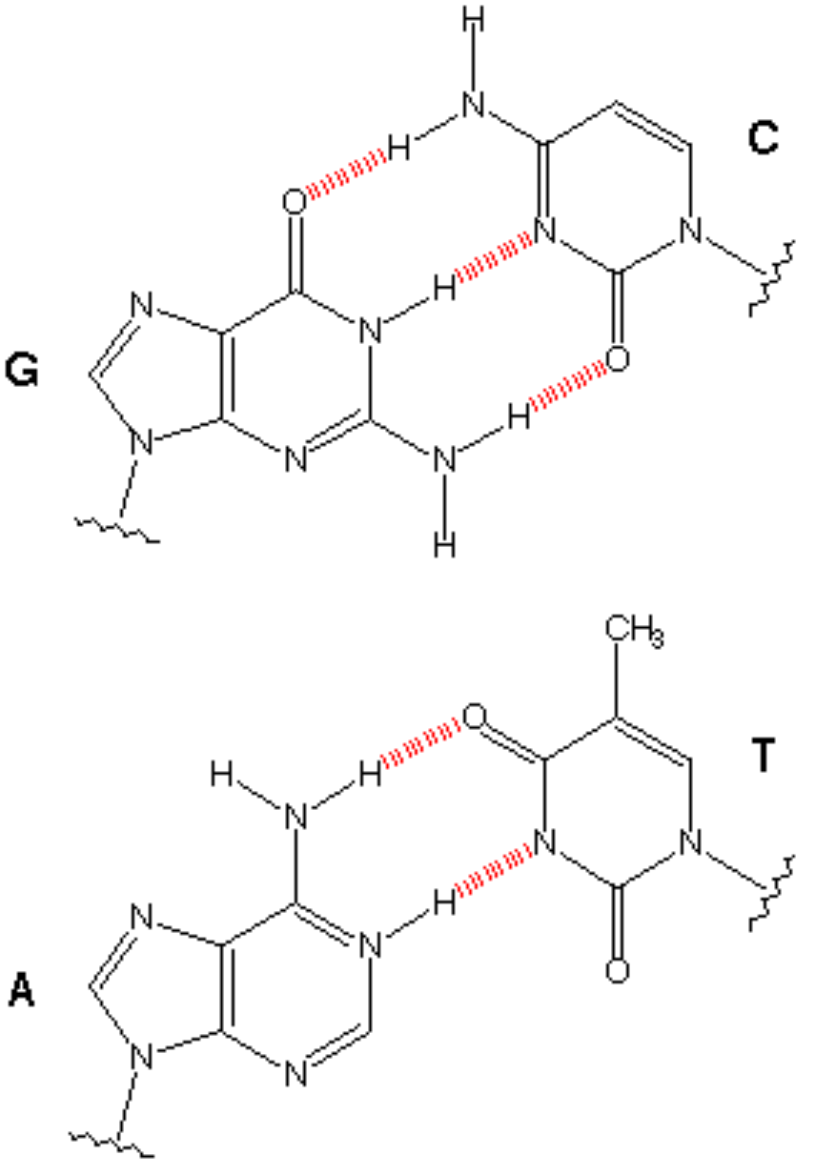
\includegraphics[scale=1]{lhex_a}}}$
        $\vcenter{\hbox{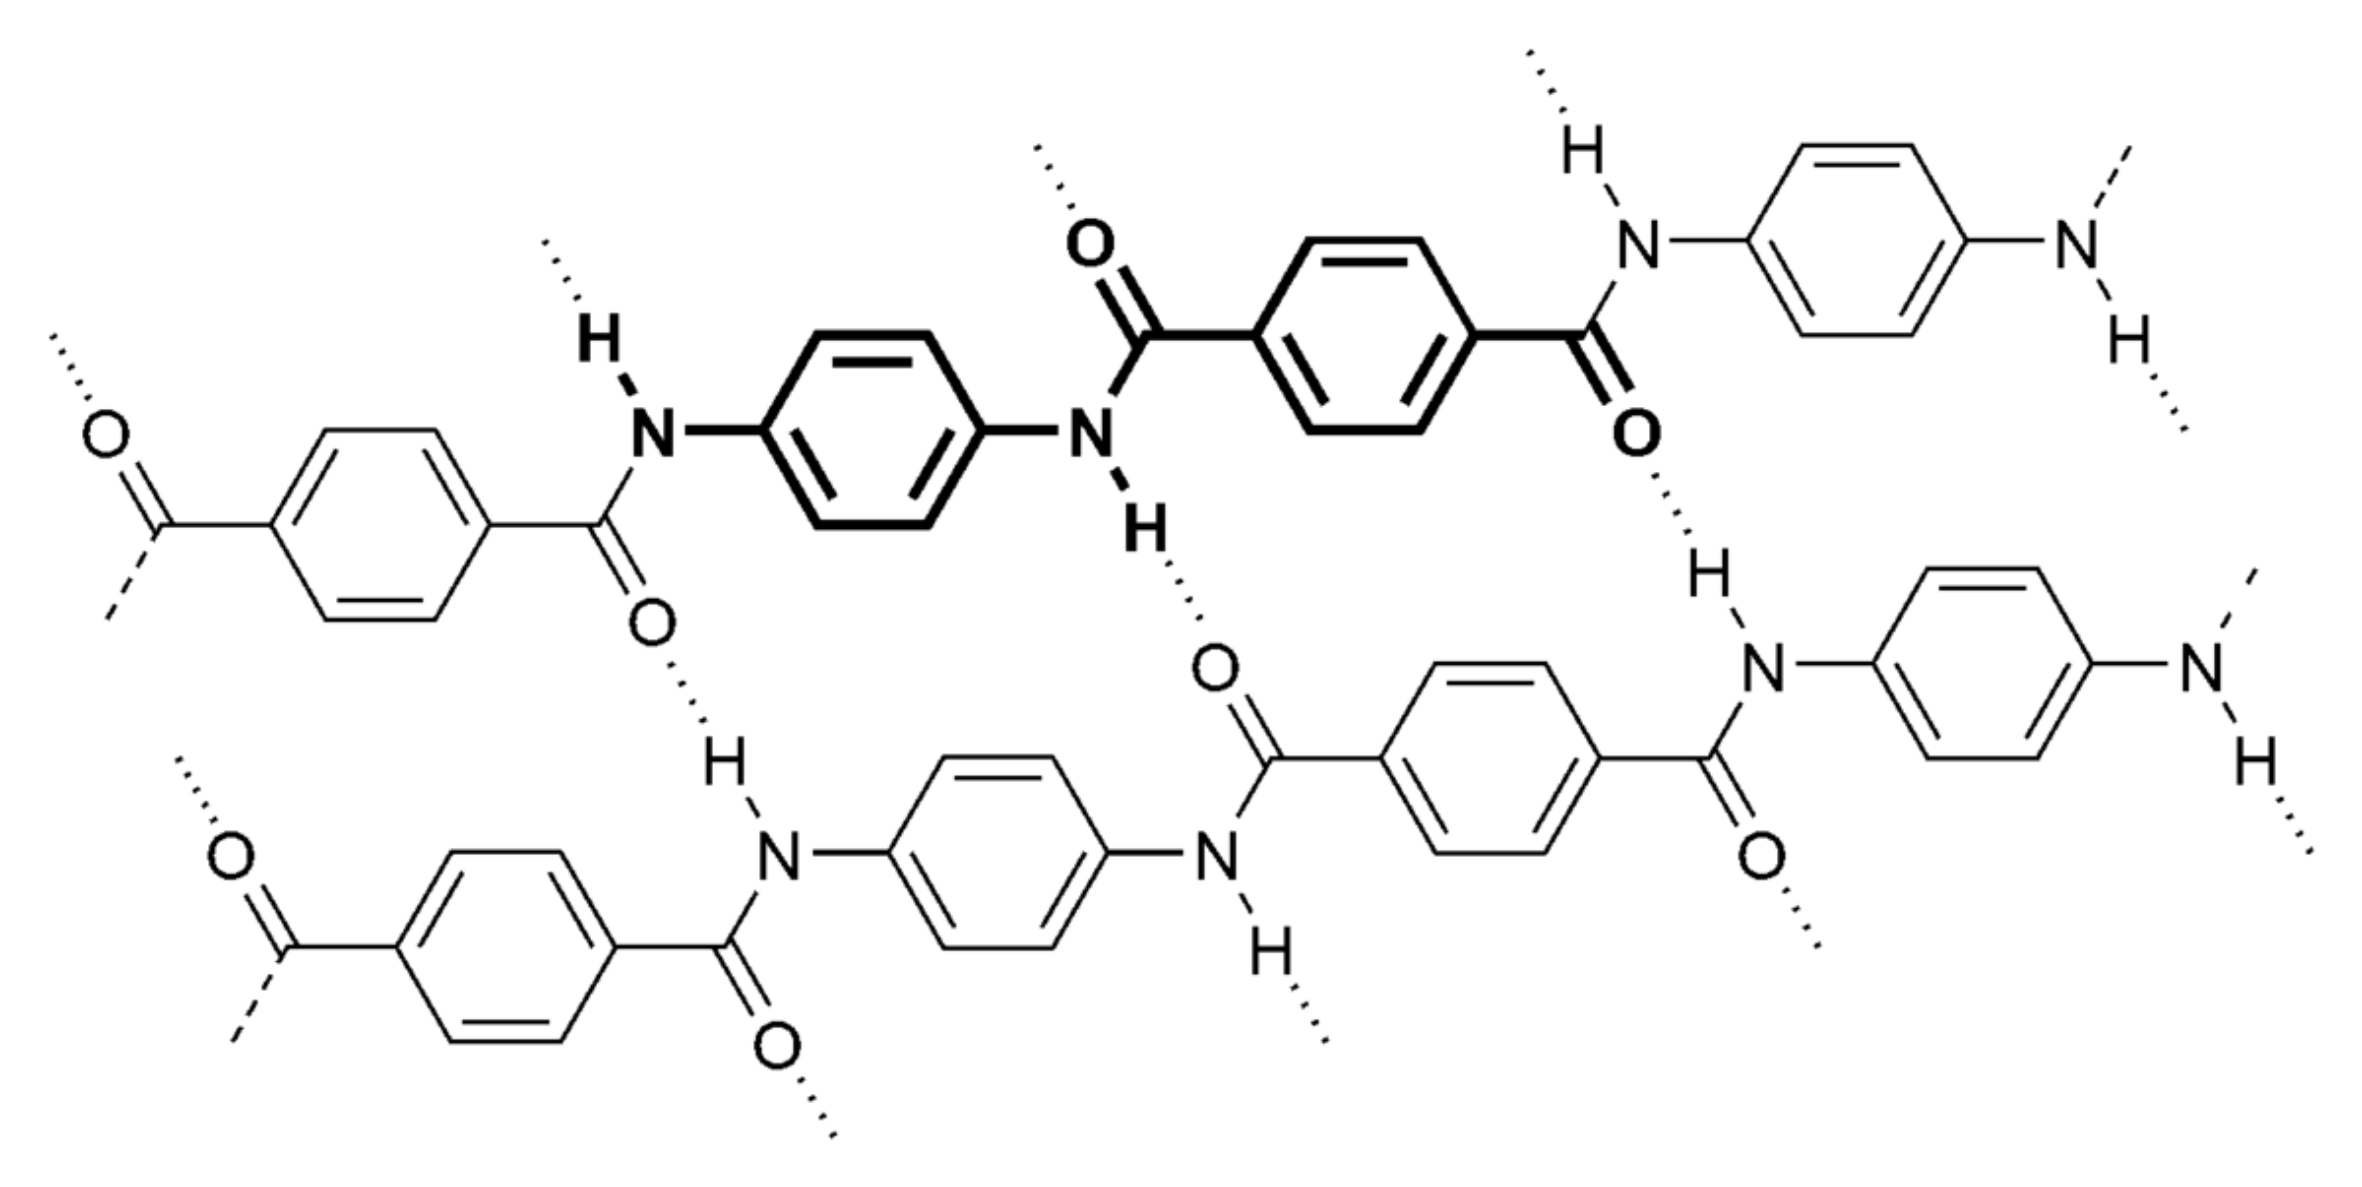
\includegraphics[scale=1]{lhex_b}}}$
    \end{center}
    \begin{itemize}
        \item Les LH expliquent la cohésion dans la double hélice de l'ADN,
            \textit{via} la correspondance entre adénine et thymine d'une
            part, et entre guanine et cytosine d'autre part.
        \item Les LH expliquent la cohésion entre les fibres de Kevlar.
        \item Les LH expliquent la haute température d'ébullition de nombreux
            composés chimiques, notamment celle de l'eau.
    \end{itemize}
\end{rexem}

\section{Solvants}
Une autre propriété macroscopique que l'on expérimente tous les jours à tous les
égard est celle des solvants, qui composent la quasi-totalité de nos
interactions physico-chimiques au quotidien. Voyons comment caractériser ces
solvants, et surtout pourquoi l'eau permet autant de réactions chimiques.

\subsection{Classement}
Les solvants sont classés selon 3 caractéristiques~:
\begin{enumerate}
    \item Leur caractère \textbf{polaire ou apolaire}~;
    \item Leur caractère \textbf{protique ou aprotique} (capable de
        liaisons hydrogène ou pas)~;
    \item Leur \textbf{pouvoir dispersant}.
\end{enumerate}

On a déjà parlé des 2 premières, présentons la troisième~:
\subsubsection{Pouvoir dispersant}
Lorsque deux ions de charges opposées $\pm q$ sont séparés d'une distance $d$
dans le vide, ils exercent l'un sur l'autre une force attractive de norme
\[F_0 = \frac{q^2}{4\pi\ep_0d^2}\]
avec $\ep_0$ la permittivité diélectrique du vide. Dans un milieu \textbf{autre
que le vide}, par exemple un \textbf{solvant}, la force reste attractive mais le
milieu modifie la norme de cette force \textit{via} sa permittivité relative
$\ep_r$~:
\[F_{\rm milieu} = \frac{q^2}{4\pi\ep_0\ep_rd^2} = F_0\times
\frac{1}{\ep_r}\]
Autrement dit, quand un solvant s'infiltre entre deux ions, le milieu entre les
deux change et ils sont moins attirés.

\begin{tdefi}{Définition~: permittivité relative}
    La \textbf{permittivité relative} d'un solvant est une constante, notée
    $\ep_r\footnote{Cette grandeur est reliée à l'indice optique d'un milieu~:
    on a $n=\sqrt{\ep_r}$.}$
    avec $\ep_r > 1$, caractérisant sa capacité à séparer deux ions.
    Plus elle est grande, plus il est \textbf{dispersant}, c'est-à-dire capable
    de séparer des charges. On a~:
    \begin{itemize}[label=$\diamond$]
        \item $01 < \ep_r < 20 \Ra$ peu dispersant~;
        \item $20 < \ep_r < 40 \Ra$ dispersant~;
        \item $40 < \ep_r \lesssim 100 \Ra$ très dispersant.
    \end{itemize}
\end{tdefi}
On dit que l'interaction entre les ions est \textit{écrantée} par le solvant.

\subsubsection{Exemple de solvants}
\begin{table}[h!]
    \centering
    \begin{threeparttable}
        \caption{Exemples de solvants polaires et apolaires.}
        \label{tab:solpoapo}
        \begin{tabular}{cccccc}
            \toprule
            Solvant & Eau\tnote{1} & Méthanol & Ammoniac & Propanone\tnote{2} &
            Cyclohexane
            \\\midrule
            \textsc{Lewis} &
            $\vcenter{\hbox{
                \cfig{[,.7]\lewis{13,O}(-[5]H)(-[7]H)}
            }}$ &
            $\vcenter{\hbox{
                \cfig{CH_3-[,.7]\lewis{26,O}-[,.7]H}
            }}$&
            $\vcenter{\hbox{
                \cfig{\lewis{2,N}(<:[5]H)(<[6]H)(-[7]H)}
            }}$&
            $\vcenter{\hbox{
            \cfig{[,.7]
                C
                (=[2]\lewis{13,O})
                (-[:-20]CH_3)
                (-[:200]CH_3)
            }}}$
            &
            $\vcenter{\hbox{\chemfig{[,.7]
                H_2C*6(-CH_2-CH_2-CH_2-CH_2-H_2C-[,,2])
            }}}$
            \\\midrule
            $\mu$ (\si{D}) &
            \num{1.85} &
            \num{1.65} &
            \num{1.30} &
            \num{2.77} &
            0
            \\
            Polarité &
            Polaire &
            Polaire &
            Polaire &
            Polaire &
            Apolaire
            \\\midrule
            Proticité &
            Protique &
            Protique &
            Protique &
            Aprotique &
            Aprotique
            \\\midrule
            $\ep_r$ &
            \num{78.5} &
            \num{32.6} &
            \num{25.0} &
            \num{20.7} &
            \num{2.1}
            \\
            Dispersant &
            Fortement &
            Oui &
            Oui &
            Oui &
            Presque pas
            \\\bottomrule
        \end{tabular}
        \begin{tablenotes}[flushleft]
            \item[1] L'eau est, pour toutes ces caractéristiques, l'un des meilleurs
                solvants sur Terre.
            \item[2] Communément appelé acétone.
        \end{tablenotes}
    \end{threeparttable}
\end{table}

\subsection{Solubilité, miscibilité}
\subsubsection{Définition}
\begin{tdefi}{Définition, sidebyside}
    \begin{center}
        \textbf{Solubilité}
    \end{center}
    La solubilité d'un \textbf{solide}, appelé soluté, est la \textbf{quantité
    maximale} qu'il est possible de \textbf{dissoudre} dans un litre de solution
    d'un solvant. Elle s'exprime en \si{g.L^{-1}} ou en \si{mol.L^{-1}}.
    \tcblower
    \begin{center}
        \textbf{Miscibilité}
    \end{center}
    On parle de miscibilité pour caractériser la capacité de \textbf{deux
    liquides} à se \textbf{mélanger} pour former une solution homogène.
\end{tdefi}

\subsubsection{Mise en solution d'espèces ioniques}
Dans l'eau, les solides ioniques se dissolvent en deux étapes\footnote{Il est
    possible qu'une étape d'ionisation intervienne en amont, où le solvant créé
des charges sur l'espèce. Il faut un solvant \textbf{très polaire} pour ça.}~:
\[
    \ce{
        NaCl\sol{}
        ->T[dissociation]
        Na+ + Cl-
        ->T[solvatation]
        Na\plus{}\aqu{} + Cl\moin{}\aqu{}
}\]
\begin{itemize}
    \litem{Dissociation}~: le solvant affaiblit les interactions à l'intérieur du
        soluté pur. Cette étape est reliée à la \textbf{permittivité} du
        solvant.
    \litem{Solvatation}~: le solvant augmente ses interactions avec le soluté. La
        qualité dépend de leurs \textbf{polarités} et de leurs
        \textbf{proticités}.
\end{itemize} \smallbreak
Notamment, si les caractéristiques du soluté et du solvant sont similaires, il
suffit de peu d'énergie/température pour que le processus se passe. Il y a de
nombreuses vidéos en
ligne\footnote{\url{https://www.youtube.com/watch?v=xdedxfhcpWo}}. Ainsi,

\begin{tror}{Conclusion, heart, sidebyside, righthand ratio=.4}
    \begin{itemize}
        \item Un solvant dissout des composés semblables~;
        \item Deux solvants semblables sont miscibles.
    \end{itemize}
    \tcblower
    \begin{center}
        \begin{bfseries}
            \fbox{Qui se ressemble s'assemble~!}
        \end{bfseries}
    \end{center}
\end{tror}

\begin{rexem}{Exemples}
    \begin{itemize}
        \item Le glucose est très soluble dans l'eau~: \SI{700}{g.L^{-1}} à
            $T_{\rm amb}$. Il est en effet protique comme l'eau et réalise de
            nombreuses liaisons hydrogènes.
        \item Le diiode est apolaire, il est donc peu soluble dans l'eau, mais
            il l'est en revanche dans le cyclohexane.
    \end{itemize}
\end{rexem}



\end{document}
